\section{Génération d'objet paramétrique~: le diamant}

Dans un premier temps, nous nous sommes attaqué au maillage des diamants.
Pour se faire, nous avons découpé l'algorithme en deux étapes principales:
\begin{itemize}
    \item Génération des points dans l'espace
    \item Génération des faces
\end{itemize}

\subsection{Génération des points}

Pour générer les points du diamant, on considère deux sommets aux extrémités du diamant, ainsi que 2 cercles sur lesquels
les points seront répartis, tout cela en fonction du nombre de facettes désiré.

{\centering 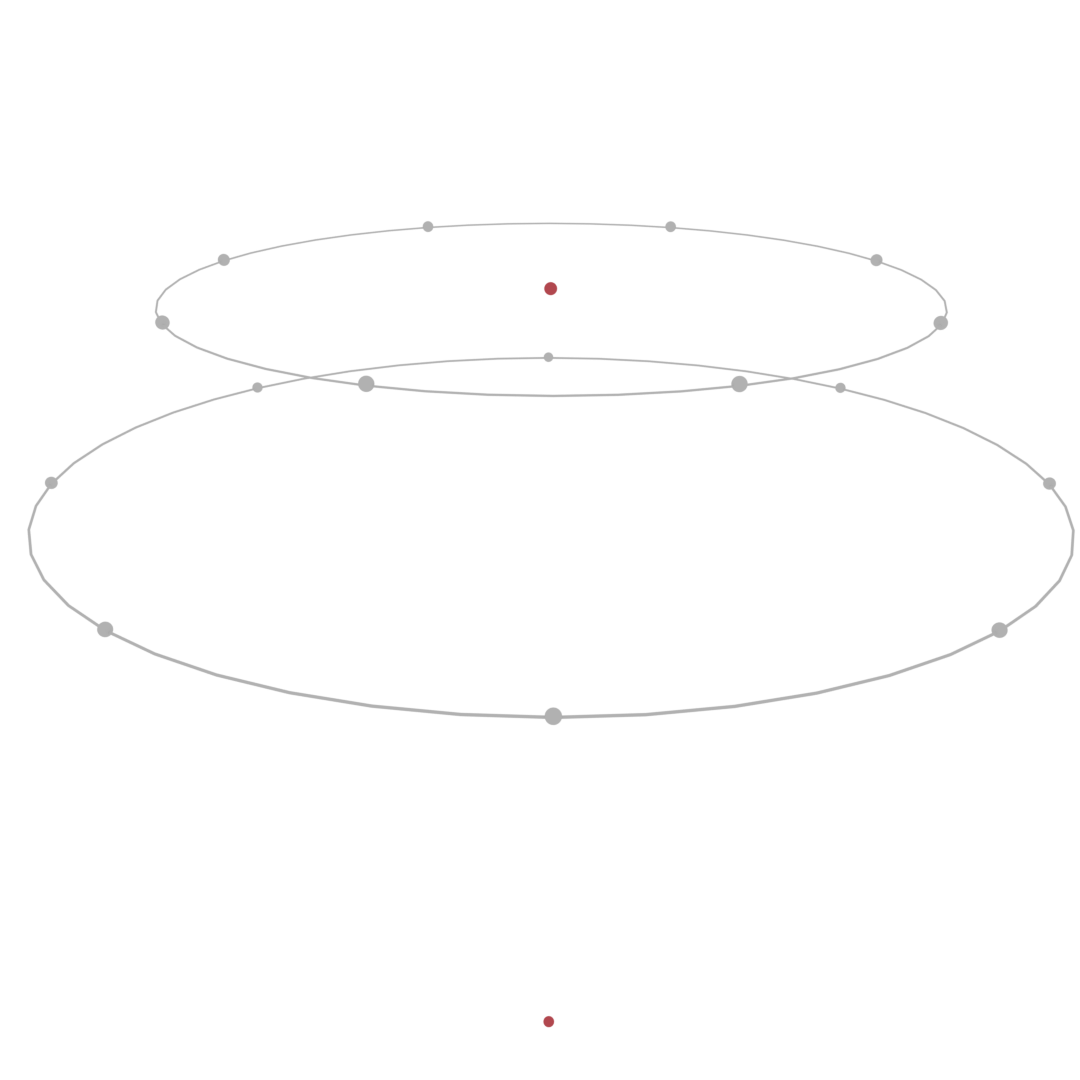
\includegraphics[width=0.7\textwidth]{Maillage/circles}}

Une fois les points placés, il ne reste plus qu'a les relier.

\subsection{Génération des faces}
Pour relier les dits points, on pourra se contenter de simples triangles, étant donné
qu'en dehors des triangles de la face supérieure, tous les autres triangles auront des normales différentes.

{\centering 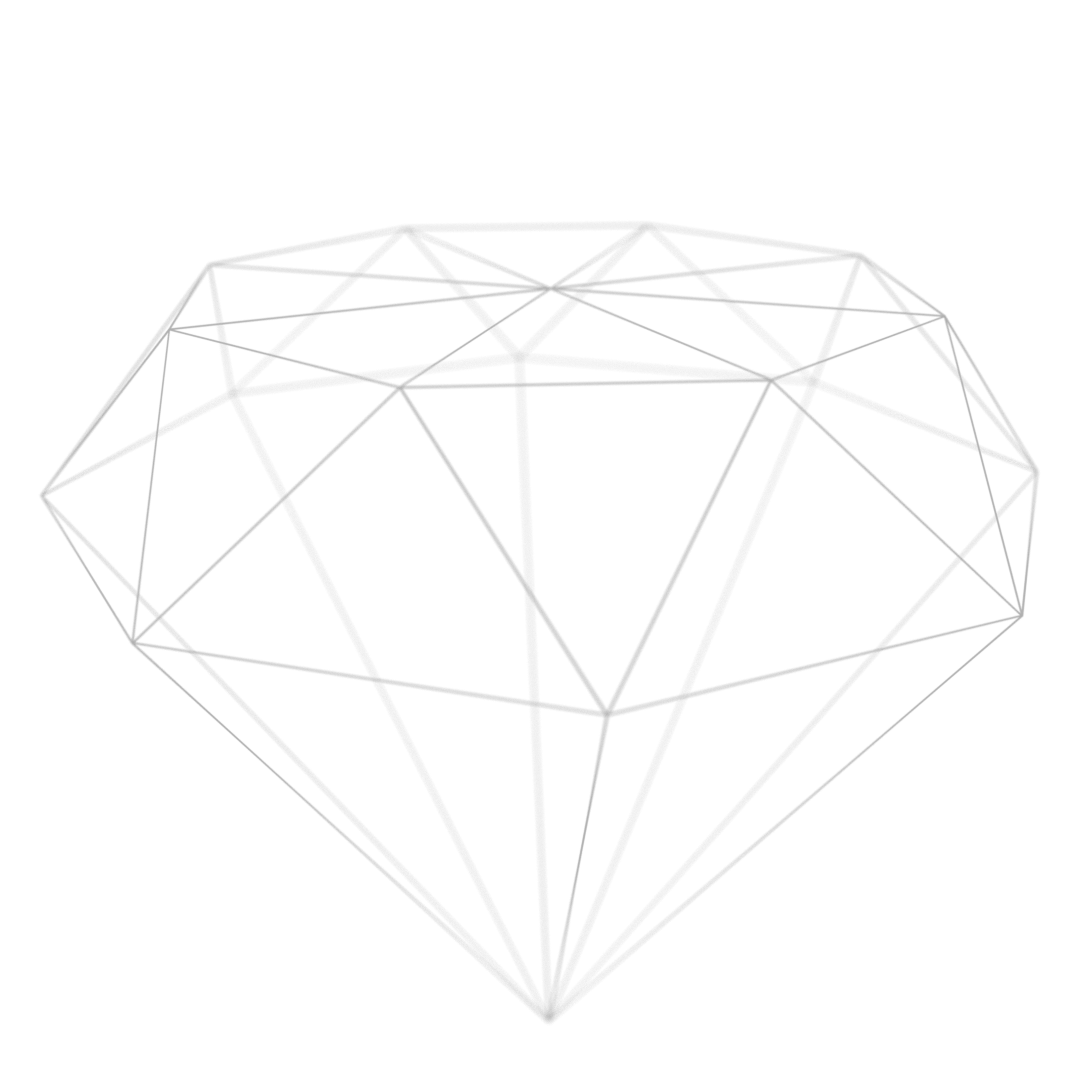
\includegraphics[width=0.7\textwidth]{Maillage/wireframe}}

Il ne nous reste alors plus qu'a calculer les normales de chaque face, ce que l'on peut faire  à l'aide d'un produit
vectoriel, en choisissant bien ses vecteurs.

La figure suivante est une petite démonstration du résultat final, avec le système d'éclairage de Phong qui
sera présenté dans la prochaine section~:

{\centering 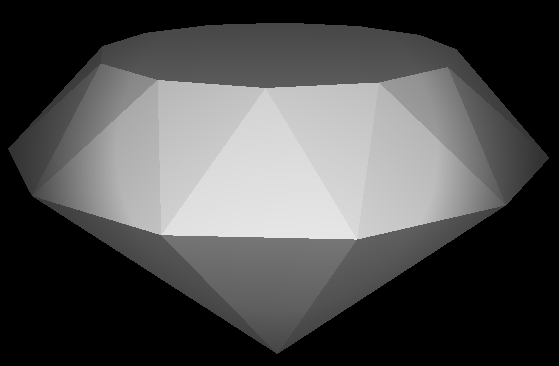
\includegraphics[width=0.7\textwidth]{Maillage/result}}

